%======================================================================
% L03b_Entropy_open.pdf
%======================================================================
\section{Entropie -- otevřené systémy}
\strana{L03b-1}

\begin{itemize}
  \item vratné procesy v uzavřených systémech:
  \[
    (*)\qquad \vzorec{\dd S = \frac{\text{đ}Q}{T} = \frac1T\,\dd U - \sum_i\frac{y_i}{T}\,\dd X_i}
  \]
  \item nevratné procesy: \quad
  $\dd S = \dfrac{\text{đ}Q}{T} + \dd S_i = \dd S_e + \dd S_i$
  \quad \begin{minipage}[t]{0.42\textwidth}\small
    $\nearrow$ tok $S$ přes hranici systému \\
    $\searrow$ nárůst entropie vnitřními procesy v systému spoj.\ s nevratností
  \end{minipage}
  \item v otevřených ($\dd N_k\neq 0$) systémech přispívá k $\dd S_e$ také \kw{konvekce entropie} a \kw{tok částic}
  $\Rightarrow$ zatím nevíme, jak s entropií v otevřených systémech zacházet
\end{itemize}

\hfill\textcolor{Red}{$\displaystyle\Big(\pdv{S}{U}\Big)_X = \frac1T$ \quad vs. \quad $\displaystyle\Big(\pdv{S}{T}\Big)_X = \;???$}

\subsection*{1) Entropie id.\ plynu v uzavřeném systému}
\[
  \frac1T = \frac{cNk_B}{U} \quad\&\quad \frac{p}{T} = \frac{Nk_B}{V}
\]
\[
  \Rightarrow\ \dd S = \frac1T\dd U + \frac pT\dd V = cNk_B\frac{\dd U}{U} + Nk_B\frac{\dd V}{V}
  \ \Rightarrow\ \vzorec{S = Nk_B\log\Big[\Big(\frac{U}{U_0}\Big)^c\Big(\frac{V}{V_0}\Big)\Big] + S_0}
\]
$\to U = U(T)$ $\Rightarrow$ můžeme také triviálně psát $\dd U = cNk_B\,\dd T$ a integrovat
\[
  \dd S = cNk_B\frac{\dd T}{T} + Nk_B\frac{\dd V}{V}
  \ \Rightarrow\ \vzorec{S = Nk_B\log\Big[\Big(\frac{T}{T_0}\Big)^c\Big(\frac{V}{V_0}\Big)\Big] + S_0}
\]
$\to$ také $S(T,V) = S(U(T),V)$, \pozor{obecně ale tyto funkce nebudou ekvivalentní!}

\pozor{!} z $(*)$ vyplývá, že entropie je \kw{přirozeně funkcí ext.\ proměnných}
\[
  \vzorec{S = S(U, X_1,\dots,X_n) \ \Leftrightarrow\ U = U(S, X_1,\dots,X_n)}
\]

\subsection*{Gibbsův paradox}
\begin{minipage}{0.42\textwidth}
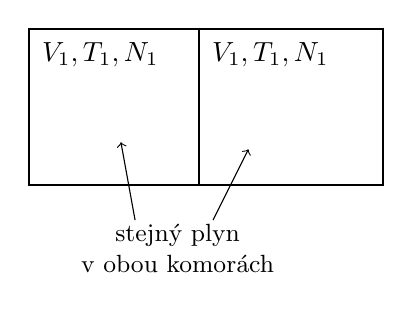
\begin{tikzpicture}[scale=0.9]
  \draw[thick] (0,0) rectangle (5,2.2);
  \draw[thick] (2.4,0) -- (2.4,2.2);
  \node[anchor=north west] at (0.05,2.15) {$V_1,T_1,N_1$};
  \node[anchor=north west] at (2.45,2.15) {$V_1,T_1,N_1$};
  \draw[->] (1.5,-0.5) -- (1.3,0.6);
  \draw[->] (2.6,-0.5) -- (3.1,0.5);
  \node[align=center,font=\small] at (2.1,-0.9) {stejný plyn \\ v obou komorách};
\end{tikzpicture}
\end{minipage}
\begin{minipage}{0.56\textwidth}
\begin{enumerate}[label=\arabic*)]
  \item systémy oddělené \hfill \textcolor{Red}{\small zde předp.\ aditivitu entropie $\downarrow$}
  \[ S^{(1)}_{\text{celk}} = 2N_1k_B\log\Big[\Big(\frac{T_1}{T_0}\Big)^c\Big(\frac{V_1}{V_0}\Big)\Big] + 2S_0 \]
  \item přepážku odstraním \\
  $\Rightarrow N_1\to 2N_1$, $V_1\to 2V_1$, $T_1\to T_1$ \quad (pouze jeden systém)
  \pozn{v originále $V_1\to 2V_2$}
\end{enumerate}
\end{minipage}

\[
  \Rightarrow S^{(2)} = 2N_1k_B\log\Big[\Big(\frac{T_1}{T_0}\Big)^c\Big(\frac{2V_1}{V_0}\Big)\Big] + \textcolor{Red}{\boxed{2}}S_0 \quad \textcolor{Red}{?}
\]
\[
  \Rightarrow S^{(2)} - S^{(1)} = 2N_1k_B\log 2 > 0 \ \Rightarrow\ \text{entropie stoupla}
\]
\begin{enumerate}[label=\arabic*),start=3]
  \item přepážku opět uzavřu $\Rightarrow$ $S\to S^{(1)}$ $\Rightarrow$ \underline{$\Delta S < 0$ beze změny stavu okolí?} \\
  $\bullet$ srov.\ případ, kdy jsou plyny v komorách různé -- potom 1) $\neq$ 3)
\end{enumerate}
\begin{itemize}
  \item argumentace není zcela přesvědčivá
  \begin{enumerate}[label=\alph*)]
    \item skutečně jsou stavy 1) a 3) ekvivalentní?
    \item co $S_0$? implicitně předp.\ extenzivitu \pozor{!}
  \end{enumerate}
\end{itemize}

%----------------------------------------------------------------------
\strana{L03b-2}
\begin{itemize}
  \item \uv{problém} je možné rozřešit, pokud \underline{postulujeme, že entropie je extenzivní}:
  \[
    S(U,V)\to S(U,V,N) \ \Rightarrow\ S(U,V,N) = Nk_B\log\Big[\Big(\frac{U}{U_0}\Big)^c\Big(\frac{V}{V_0}\Big)\Big] + \phi(N)
  \]
  \& funkci $\phi(N)$ určíme z požadavku na extenzivitu
  \item \kw{extenzivita}: homogenita 1.\ řádu
  \[ \vzorec{S(\lambda U,\lambda V,\lambda N) = \lambda S(U,V,N)} \]
  \item $S(\lambda U,\lambda V,\lambda N) = \lambda Nk_B\log\Big[\lambda^{c+1}\Big(\frac{U}{U_0}\Big)^c\Big(\frac{V}{V_0}\Big)\Big] + \phi(\lambda N)$
  \[
    \Rightarrow\ \phi(\lambda N) = -\lambda Nk_B\log\Big(\lambda^{c+1}\Big(\frac{N}{N_0}\Big)^{c+1}\Big) + \lambda Ns_0
  \]
\end{itemize}
\[
  \vzorec{\Rightarrow\ S(U,V,N) = Nk_B\log\Big[\Big(\frac{U}{U_0}\Big)^c\Big(\frac{V}{V_0}\Big)\Big(\frac{N_0}{N}\Big)^{c+1}\Big] + Ns_0} \qquad (+)
\]
\begin{enumerate}[label=\arabic*)]
  \item $S_1 = 2\Big\{Nk_B\log\Big[\Big(\frac{T_1}{T_0}\Big)\Big(\frac{V_1}{V_0}\Big)\Big(\frac{N_0}{N}\Big)\Big] + Ns_0\Big\}$
  \item $S_2 = (2N)k_B\log\Big[\Big(\frac{T_1}{T_0}\Big)\Big(\frac{2V_1}{V_0}\Big)\Big(\frac{N_0}{2N}\Big)\Big] + (2N)s_0$
  \hfill $\Rightarrow\ S_1 = S_2$
\end{enumerate}
$\to$ \kw{extenzivita} je skutečně \underline{dodatečný postulát}; Clausiova (ne)rovn.\ vedoucí k definici entropie se na otevřené systémy nevztahuje

\begin{priklad}[Př.\ \#2]
\begin{minipage}{0.45\textwidth}
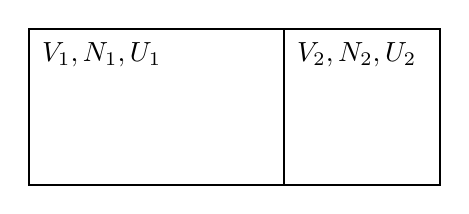
\begin{tikzpicture}[scale=0.9]
  \draw[thick] (0,0) rectangle (5.8,2.2);
  \draw[thick] (3.6,0) -- (3.6,2.2);
  \node[anchor=north west] at (0.05,2.15) {$V_1,N_1,U_1$};
  \node[anchor=north west] at (3.65,2.15) {$V_2,N_2,U_2$};
\end{tikzpicture}
\end{minipage}
\begin{minipage}{0.53\textwidth}
\begin{itemize}[nosep]
  \item předp.\ opět aditivitu entropie \\
  $\to$ jistě rozumný předpoklad minimálně pro oddělené/neinteragující podsystémy
  \item opět předp.\ stejné plyny
\end{itemize}
\end{minipage}

\begin{enumerate}[label=\arabic*)]
  \item systémy odděleny
  \[
    \Rightarrow S = N_1k_B\log\Big[\Big(\frac{U_1}{U_0}\Big)^c\Big(\frac{V_1}{V_0}\Big)\Big] + S_{01}
    + N_2k_B\log\Big[\Big(\frac{U_2}{U_0}\Big)^c\Big(\frac{V_2}{V_0}\Big)\Big] + S_{02}
  \]
  \item v přepážce vyvrtáme otvor
  \begin{itemize}[nosep]
    \item je-li malý, aditivita entropie bude stále dobrá aproximace
    \item systémy si začnou vyměňovat částice (a energii) $\Rightarrow S\nearrow$
  \end{itemize}
\end{enumerate}
\underline{OTÁZKA}: Jaká bude nová rovnováha, která se ustaví? \\
\underline{ODPOVĚĎ}: Bude odpovídat \kw{maximu entropie} za daných okraj.\ podmínek, neboli bude splňovat vazby
\begin{itemize}[nosep]
  \item $N_1' + N_2' = N_1 + N_2 = N$ \ \& \ $U_1' + U_2' = U_1 + U_2 = U$ \\
  (částice ani energie se nemohou ztratit ani vytvořit)
  \item podmínka maxima: \quad $\delta S = 0$ \ $\Leftarrow$ \ $\Delta S\geq 0$ v izol.\ systému
\end{itemize}
\end{priklad}

%----------------------------------------------------------------------
\strana{L03b-3}
\begin{minipage}{0.68\textwidth}
\begin{align*}
  \delta S &= \delta N_1k_B\log\Big[\Big(\frac{U_1}{U_0}\Big)^c\Big(\frac{V_1}{V_0}\Big)\Big] + cN_1k_B\frac{\delta U_1}{U_1} \\
  &\quad + \delta N_2k_B\log\Big[\Big(\frac{U_2}{U_0}\Big)^c\Big(\frac{V_2}{V_0}\Big)\Big] + cN_2k_B\frac{\delta U_2}{U_2}
\end{align*}
\end{minipage}
\begin{minipage}{0.3\textwidth}
\& \quad $\delta U_2 = -\delta U_1$ \\
\phantom{\& \quad} $\delta N_2 = -\delta N_1$
\end{minipage}
\[
  0 = ck_B\Big(\frac{N_1}{U_1} - \frac{N_2}{U_2}\Big)\delta U_1 + k_B\log\Big[\Big(\frac{U_1}{U_2}\Big)^c\Big(\frac{V_1}{V_2}\Big)\Big]\delta N_1
\]
\[
  \Rightarrow\ 1)\ \frac{U_1'}{U_2'} = \frac{N_1'}{N_2'} \qquad
  2)\ \Big(\frac{U_1'}{U_2'}\Big)^c\Big(\frac{V_1}{V_2}\Big) = 1 \ \overset{(1)}{\Rightarrow}\ N_1'^{\,c}V_1 = N_2'^{\,c}V_2
\]
\[
  \Rightarrow\ \boxed{N_2' = N_1'\Big(\frac{V_1}{V_2}\Big)^{1/c}} \quad\Leftrightarrow\quad V\nearrow\ \Rightarrow\ N\searrow \quad \text{\tikz[baseline=0pt]\draw[Red,thick,-{Stealth}] (0,0.35) -- (0.18,0.12) -- (0.06,0.14) -- (0.22,-0.15);}
\]

\underline{Oprava:} nechť je entropie extenzivní $(+)$
\[
  S_i(U,V,N) = N_ik_B\log\Big[\Big(\frac{U_i}{U_0}\Big)^c\Big(\frac{V_i}{V_0}\Big)\Big(\frac{N_0}{N_i}\Big)^{c+1}\Big] + N_is_0,
  \qquad S = S_1 + S_2
\]
\[
  \Rightarrow\ \delta S_i = \Big\{k_B\log\big[(\ \ )\big] - (c+1)k_B + s_0\Big\}\delta N_i + ck_B\frac{N_i}{U_i}\delta U_i
\]
\begin{itemize}
  \item opět $\delta U_2 = -\delta U_1$; \ $\delta N_2 = -\delta N_1$
  \[
    \Rightarrow\ 1)\ \frac{U_1'}{N_1'} = \frac{N_1'}{N_2'} \quad (\delta U) \pozn{tak v originále; míněno $U_1'/U_2' = N_1'/N_2'$}
  \]
  \[
    2)\ \Big(\frac{U_1'}{U_2'}\Big)^c\Big(\frac{V_1}{V_2}\Big)\Big(\frac{N_2'}{N_1'}\Big)^{c+1} = 1
    \ \overset{(1)}{\Rightarrow}\ \frac{V_1N_2}{V_2N_1}\ \Rightarrow\ \vzorec{N_2' = N_1\Big(\frac{V_2}{V_1}\Big)} \quad \checkmark
  \]
  \item vidíme, že postulovat extenzivitu entropie se zdá být rozumné:
  \begin{enumerate}[label=\arabic*)]
    \item dostáváme očekávané chování v některých intuitivních případech
  \end{enumerate}
\end{itemize}
\begin{center}
\itshape (Feynman: A paradox is a conflict between reality and your feeling of what reality ought to be.)
\end{center}

%----------------------------------------------------------------------
\strana{L03b-4}
\begin{enumerate}[label=\arabic*),start=2]
  \item $U$ extenzivní, $T$ intenzivní $\Rightarrow$ vztahy $\dd S = \dfrac{\text{đ}Q}{T}$ a $\dd U = T\dd S$ se zdají indukovat extenzivitu $S$ \\
  (ovšem zde opět stavíme na sporném argumentu; odvození bylo pro uzavřené systémy) \\
  $\to$ možná je extenzivita nutná pro konzistenci teorie? Zdá se, že ne, je možné konstruovat TD i bez tohoto předpokladu
  \item extenzivita $S$ není tak intuitivní jako extenzivita $U$ -- podobně jako $T$, $S$ není přímým projevem nějaké mikroskopické vlastnosti složek látky, je to charakteristika makrostavu, na mikro úrovni nemá $S$ žádný smysl
\end{enumerate}
\begin{veta}[Extenzivita entropie]
$\Rightarrow$ \kw{extenzivitu} je opravdu třeba chápat jako \underline{dodatečný axiom}, který umožní rozšířit platnost definice na otevřené systémy

\textcolor{NavyBlue}{\small Někdy se požadavek na extenzivitu uvádí jako 4.\ TDZ/princip: všechny TD veličiny jsou buď extenzivní, nebo intenzivní}
\end{veta}

\subsection*{Diferenciál extenzivní entropie}
\begin{itemize}
  \item $N$ je plnohodnotná stavová proměnná, v principu nezávislá
\end{itemize}
\[
  \Rightarrow\quad
  \vzorec{\begin{aligned}
    \dd U &= T\dd S + \sum_i y_i\dd X_i + \overbrace{\sum_j\mu_j\dd N_j}^{\textcolor{NavyBlue}{\text{Gibbs -- chemická práce}}} \\
    &\Downarrow \\
    \dd S &= \frac1T\dd U - \sum_i\frac{y_i}{T}\dd X_i - \sum_j\frac{\mu_j}{T}\dd N_j
  \end{aligned}}
  \qquad
  \begin{minipage}{0.28\textwidth}
    $N_j$ \dots\ počet částic $j$-té složky (chemické komp., fáze, \dots)
  \end{minipage}
\]
\begin{itemize}
  \item \underline{$\mu_\ell(S,X_1,\dots,X_n,N_1,\dots,N_\ell)$} \dots\ (elektro)\kw{chemický potenciál}
  \[
    \vzorec{\mu_j = \Big(\pdv{U}{N_j}\Big)_{S,X_i,N_{p\neq j}}}
    \quad\dots\ \begin{minipage}{0.45\textwidth}energie potřebná k přidání jedné částice do systému při \underline{zach.\ entropie} a ost.\ ext.\ veličin\end{minipage}
  \]
\end{itemize}

%----------------------------------------------------------------------
\strana{L03b-5}
\begin{itemize}
  \item[$\to$] obvykle platí $\mu_j < 0$ \dots\ přidáme-li částici do systému při $\dd U = 0$, potom entropie typicky vzroste \\
  $\Rightarrow$ tento nárůst je třeba kompenzovat odebráním tepla $\Leftrightarrow$ $\dd U < 0$
  \item[$\to$] $\mu > 0$ možné pouze pro odpuzující se částice
  \item[$\to$] $S$ je v kontextu $\mu$ zjevně velmi významná: v id.\ plynu $\mu\neq 0$, přestože částice neinteragují $\Rightarrow$ \pozor{chem.\ práce je důsledkem pouze entropie!}
\end{itemize}

%----------------------------------------------------------------------
\strana{L03b-6}
\subsection{Entropie a statistika -- Boltzmannova entropie}
\begin{itemize}
  \item uvolnění vazeb v izolovaném systému vede k nárůstu entropie
  \begin{itemize}
    \item[$\to$] uvolnění vazeb zároveň zvětšuje dostupný stavový prostor $\Leftrightarrow$ počet dostupných mikrostavů
    \item[$\to$] méně vazeb $\equiv$ menší uspořádanost
  \end{itemize}
  \item rovnovážný stav je v nějakém smyslu nejvíce pravděpodobný -- mikrostavy přecházejí jeden na druhý, ale makrostav se nemění \\
  $\overset{?}{\Rightarrow}$ po uvolnění vazeb systém \uv{prozkoumává} i nově dostupné mikrostavy; směřování k rovnováze ($S\nearrow$) lze interpretovat jako proces, kdy \uline{systém přechází od makrostavů odpovídajících malému počtu mikrostavů k těm charakterizovaným větším počtem mikrostavů} (více pravděpodobným) \\
  $\to$ přechod zpět k méně pravděp.\ makrostavu není vyloučen, je jen nepravděpodobný ($\Rightarrow$ fluktuace) -- \kw{mikroskopická interpretace nevratnosti}
\end{itemize}
$\Rightarrow$ má smysl \underline{asociovat entropii s pravděpodobností makrostavu?}

\begin{itemize}
  \item pst makrostavu -- $W$ \dots\ \emph{Wahrscheinlichkeit} \\
  \quad $W\propto$ počet mikrostavů asociovaných s daným makrostavem ($\Rightarrow$ celé číslo)
\end{itemize}

%----------------------------------------------------------------------
\strana{L03b-7}
\begin{itemize}
  \item hledám $S = f(W)$ s požadavky:
  \begin{enumerate}[label=\arabic*)]
    \item aditivita pro nezávislé systémy (v zásadě extenzivita, ale je to trochu slabší požadavek)
    \item pravděpodobnost toho, že nastanou dva nezávislé jevy najednou, je rovna součinu jejich jednotlivých pstí
  \end{enumerate}
\end{itemize}

\begin{minipage}[t]{0.45\textwidth}
\begin{align*}
  \Rightarrow\ f(W_1W_2) &= f(W_1) + f(W_2) && \partial/\partial W_1 \\
  W_2f'(W_1W_2) &= f'(W_1) && \partial/\partial W_2 \\
  W_1W_2f''(W_1W_2) &+ f'(W_1W_2) = 0 &&
\end{align*}
\[ \Downarrow \]
\end{minipage}
\begin{minipage}[t]{0.53\textwidth}\color{NavyBlue}
\vspace{10mm}
\[ \overset{\text{\textcircled{\tiny 1}}}{\Downarrow} \]
\[ xf''(x) + f'(x) = 0 \qquad \Big/\!\!\int\dd x \]
\begin{align*}
  \int xf''(x)\dd x + f(x) = K &= xf'(x) - \int f'(x)\dd x + f(x) \\
  &= xf'(x) - f(x) + f(x)
\end{align*}
\[ \Rightarrow f'(x) = \frac Kx \ \Rightarrow\ f(x) = K\log x + f_0 \]
\end{minipage}

\begin{veta}[Boltzmannova entropie]
\[ \vzorec{S = K\log W} + S_0 \quad\Leftarrow \]
(ve skut.\ ji takto napsal Planck)
\end{veta}
\begin{itemize}
  \item můžeme brát $S_0 = 0$?
  \[ S = K\log\Big(\frac{W}{W_0}\Big) \ \to\ \Delta S = S(1) - S(2) = K\log\Big(\frac{W_1}{W_2}\Big) \]
  \quad $\Rightarrow$ aditivní konstanta vypadne
  \item více u 3.\ TDZ -- lze $S(T\to 0)\to 0$?
  \item hlubší úvahy na téma $W_0$ vedou také k úvahám o subjektivnosti $S$ -- záleží na citlivosti experimentu, jaké stupně volnosti ještě rozliší (atomy, molekuly $\to p, n, e^-$ $\to$ chromodynamika, \dots?)
\end{itemize}

%----------------------------------------------------------------------
\strana{L03b-8}
\begin{priklad}[Volná expanze do vakua]
$V\to 2V$ \\
$\to$ po ustavení rovnováhy je pst., že danou částici najdu v původním objemu $V$, jen poloviční v porovnání s pstí, že ji najdu v celém objemu $2V$
\[ \Rightarrow\ W_2/W_1 = 2^N \ \Rightarrow\ \Delta S = KN\log 2 \]
$\Rightarrow$ porovnáním s TD entropií id.\ plynu
\[ \Delta S = Nk_B\log\Big(\frac{2V}{V}\Big) = Nk_B\log 2 \]
\end{priklad}
dostaneme
\[ \vzorec{S = k_B\log W} \qquad \Big(= k_B\log\frac{W}{W_0}\Big) \]
\begin{itemize}
  \item jak počítat $W$ -- viz poslední třetina kurzu
  \item v tuto chvíli jen víme, že $W$ musí být funkcí ext.\ TD proměnných
\end{itemize}
\[
  S(U,X_1,\dots,X_n,N_1,\dots,N_\ell) = k_B\log W(U,\dots)
  \ \Rightarrow\ \vzorec{W = \exp\Big(\frac{1}{k_B}S(U,\dots)\Big)}
\]

\underline{Pozn:}
\begin{itemize}
  \item $S$ je míra počtu mikrostavů kompatibilních s makroskopickou znalostí o systému \\
  $\Rightarrow$ v nějakém smyslu je \kw{mírou chybějící informace} -- tedy té informace, která nám při plné specifikaci makrostavu chybí k plné specifikaci mikrostavu
\end{itemize}

%----------------------------------------------------------------------
\strana{L03b-9}
\begin{itemize}
  \item je-li $S$ v nějakém smyslu subjektivní (závisí na rozlišovací schopnosti měření), je také míra disipované energie ztracené ve formě tepla závislá na naší schopnosti tuto energii převézt zpět na práci?
\end{itemize}
\quad $\Rightarrow$ \underline{úvahy o Maxwellovu démonu} \hfill \textcolor{NavyBlue}{\small viz např.\ Luscombe, Ch.\ 12}

\quad $\Rightarrow$ \underline{Szilardův stroj} a \kw{entropie informace} $\leftarrow$ \underline{Shannon}

\begin{center}
\begin{tikzpicture}[scale=0.85,>=Stealth]
  % (1)
  \node at (3.2,8.4) {(1)};
  \draw (4,7.6) rectangle (8,9.2);
  \fill (5.2,8.5) circle (2pt);
  \draw[->] (6,7.5) -- (6,7.2);
  \node[align=center,font=\small] at (6,6.8) {vložím přepážku \\ a podívám se, kde je částice};
  \draw[->] (4.6,6.3) -- (3.8,5.8);
  \draw[->] (7.4,6.3) -- (8.2,5.9);
  % (2a)
  \node at (-0.7,4.6) {(2a)};
  \draw (1,3.8) rectangle (5,5.4);
  \draw (3.1,3.8) -- (3.1,5.4);
  \fill (2.3,4.7) circle (2pt);
  \draw[->] (2.3,4.7) -- (3.05,5.05);
  \draw (3.1,4.55) -- (0.45,4.55);
  \draw (0.45,4.4) circle (0.18);
  \draw (0.27,4.4) -- (0.27,3.6);
  \node[draw,font=\scriptsize,inner sep=2pt] at (0.27,3.4) {$M$};
  \draw[->] (2.1,2.9) -- (2.2,3.75);
  \node[align=center,font=\small] at (2.1,2.5) {$Q$ \\ (lázeň)};
  % (2b)
  \node at (13,4.6) {(2b)};
  \draw (7,3.8) rectangle (11,5.4);
  \draw (9.1,3.8) -- (9.1,5.4);
  \fill (9.7,4.4) circle (2pt);
  \draw[->] (9.7,4.4) -- (9.15,4.65);
  \draw (9.1,4.85) -- (11.5,4.85);
  \draw (11.5,4.7) circle (0.18);
  \draw (11.68,4.7) -- (11.68,3.9);
  \node[draw,font=\scriptsize,inner sep=2pt] at (11.68,3.7) {$M$};
  \draw[->] (10.1,2.9) -- (10.1,3.75);
  \node[align=center,font=\small] at (10.1,2.5) {$Q$ \\ (lázeň)};
  % (3)
  \draw[->] (3.6,3.4) -- (5.6,2.2);
  \draw[->] (8.4,3.4) -- (6.8,2.2);
  \node at (4.3,1.3) {(3)};
  \draw (5,0.5) rectangle (9,2.1);
  \fill (7.9,1.1) circle (2pt);
\end{tikzpicture}
\end{center}

$\Rightarrow$ systém vykonal práci a přitom pouze čerpal teplo z lázně, vrátil se do pův.\ stavu $(3) = (1)$
\begin{itemize}
  \item ideální plyn (pro $N = 1$)
  \[ W = k_BT\log 2 \ \Rightarrow\ \Delta S = -\frac QT = -k_B\log 2 \]
\end{itemize}
$\Rightarrow$ \pozor{do systému je třeba započítat i pozorovatele, ten si pamatuje, kde byla částice ve (2)}

%----------------------------------------------------------------------
\strana{L03b-10}
$\Rightarrow$ podle Szilarda je s tím spojen nárůst entropie pozorovatele \quad $\Delta S = k_B\log 2$ \quad ($2\leftrightarrow$ dvě možnosti)
\begin{itemize}
  \item[--] Szilardův stroj byl experimentálně realizován! \\
  (2010, 2014 -- viz Luscombe str.\ 177; refs.\ [73,74])
\end{itemize}

\underline{Shannon} -- 1948 -- kvantifikoval míru informace funkcí, která má vlastnosti entropie:
\[
  \vzorec{H(\{p_i\}) = -K\sum_{i=1}^n p_i\log p_i} \qquad (*)
\]
$\Rightarrow$ \kw{Shannonova entropie}
\[
  \text{\pozor{!}}\ p_i = \frac1n\ \ \forall i \ \Rightarrow\ H\Big(\Big\{\frac1n,\dots,\frac1n\Big\}\Big) = K\log n \ \text{\pozor{!}}
\]

\begin{minipage}{0.75\textwidth}\color{NavyBlue}
\begin{itemize}
  \item požadavky na $H$ vedoucí k $(*)$
  \item lze odvodit z Boltzmannovy entropie (myšlenkovým) procesem \underline{coarse graining} (dělení id.\ plynu na \uv{podobjemy}; viz také mikrokanonický $\to$ kanonický soubor)
\end{itemize}
\end{minipage}
\ \textcolor{NavyBlue}{$\left.\rule{0pt}{12mm}\right\}$ \begin{tabular}{l}kurz\\ stat.\\ fyziky\end{tabular}}

